\chapter{分治法}

二分查找,快速排序,归并排序,都属于分治法(Divide and Conquer)。

\section{棋盘覆盖} %%%%%%%%%%%%%%%%%%%%%%%%%%%%%%
\subsubsection{描述}
在一个$2^k \times 2^k(1 \leq k \leq 100)$的棋盘中,恰有一个方格被黑色覆盖,其他为白色。用黑色的L型牌(如图~\ref{fig:lplate}所示为4种L型牌),去覆盖棋盘中所有的白色方格,黑色方格不能被覆盖,且任意两个L型牌不能重叠(即不重不漏)。求所需L型牌的总数。

\begin{center}
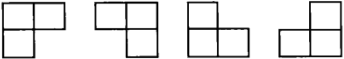
\includegraphics{lplate.png}\\
\figcaption{4种L型牌}\label{fig:lplate}
\end{center}

\subsubsection{输入}
第一行包含一个整数T,表示有T组测试用例。

每一组测试用例占用一行,包含一个整数k。

\subsubsection{输出}
所需L型牌的总数

\subsubsection{样例输入}
\begin{Code}
3
1
2
3
\end{Code}

\subsubsection{样例输出}
\begin{Code}
1
5
21
\end{Code}

\subsubsection{分析}
本题的棋盘是$2^k \times 2^k$,很容易想到用分治法。把棋盘切成4块,则每一块都是$2^{k-1} \times 2^{k-1}$的。有黑格的那一块可以递归解决,但其他3块并没有黑格子,应该怎么办呢?可以构造出一个黑格子,如图~\ref{fig:chessboard}所示,在中心放一个L型牌,其它3块也变成了子问题。递归边界不难得出,当$k=1$时1块L型牌就够了。
\begin{center}
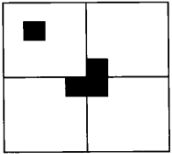
\includegraphics{chessboard.png}\\
\figcaption{棋盘覆盖问题的递归解法}\label{fig:chessboard}
\end{center}

本题只需要求总数,不需要求具体怎么摆放,因此简化很多。根据上面的思路,设$f(k)$表示棋盘是$2^k \times 2^k$时所需L型牌的总数,可得递推公式$f(k)=4f(k-1)+1$。

注意,$2^100$是一个很大的数,本题需要处理大数,见\S \ref{sec:bigintmul}节。

\subsubsection{代码}
\begin{Codex}[label=chessboard_cover.c]
#include<stdio.h>
#include<string.h>

#define MAXK 100

/* 一个数组元素表示4个十进制位,即数组是万进制的 */
#define BIGINT_MOD 10000
#define MOD_LEN 4
#define MAX_LEN (61/MOD_LEN+1)  /* 整数的最大位数, 10^x > 4^100 */

int  d[MAXK][MAX_LEN * 2];  /* d[k-1] = f(k) */

/**
 * @brief 打印大整数.
 * @param[in] x 大整数,用数组表示,低位在低地址
 * @param[in] n 数组x的长度
 * @return 无
 */
void bigint_print(const int x[], const int n) {
    int i;
    int start_output = 0;  /* 用于跳过前导0 */
    for (i = n - 1; i >= 0; --i) {
        if (start_output) {  /* 如果多余的0已经都跳过,则输出 */
            printf("%04d", x[i]);
        } else if (x[i] > 0) {
            printf("%d", x[i]);  /* 本题输出比较坑爹,最高位数字有前导0 */
            start_output = 1; /* 碰到第一个非0的值,就说明多余的0已经都跳过 */
        }
    }

    if(!start_output) printf("0");  /* 当x全为0时 */
}

/**
 * @brief 计算f(k) = 4f(k-1)+1,与大整数乘法很类似.
 * @param[in] x x
 * @param[in] y y
 * @param[out] z z=x*y+1
 * @return 无
 */
void bigint_mul_small(const int x[], const int y, int z[]) {
    int i;
    for (i = 0; i < MAX_LEN * 2; i++) z[i] = 0;

    z[0] = 1;

    for (i = 0; i < MAX_LEN; i++) z[i] += x[i] * y;
    
    for (i = 0; i < MAX_LEN * 2; i++) {  /* 统一处理进位问题 */
        if (z[i] >= BIGINT_MOD) {  /* 看是否要进位 */
            z[i+1] += z[i] / BIGINT_MOD;  /* 进位 */
            z[i] %= BIGINT_MOD;
        }
    }
}

int main() {
    int k, T;
    d[0][0] = 1;
    for (k = 2; k <= 100; k++) bigint_mul_small(d[k-2], 4, d[k-1]);

    scanf("%d", &T);
    while(T-- > 0) {
        scanf("%d", &k);
        bigint_print(d[k - 1], MAX_LEN * 2);
        printf("\n");
    }
    return 0;
}
\end{Codex}

\subsubsection{相关的题目}
与本题相同的题目:
\begindot
\item 《算法竞赛入门经典》\footnote{刘汝佳,算法竞赛入门经典,清华大学出版社,2009}第148页8.3.1节
\item 《计算机算法设计与分析(第3版)》\footnote{王晓东, 计算机算法设计与分析(第3版), 电子工业出版社, 2007}第19页2.6节
\item NYOJ 45 棋盘覆盖, \myurl{http://acm.nyist.net/JudgeOnline/problem.php?pid=45}
\myenddot

与本题相似的题目:
\begindot
\item POJ 2495 Incomplete chess boards, \myurl{http://poj.org/problem?id=2495}
\myenddot


\section{循环赛日程表} %%%%%%%%%%%%%%%%%%%%%%%%%%%%%%
\subsubsection{描述}
有$2^k$个运动员参加循环比赛,需要设计比赛日程表。要求如下:

\begindot
\item 每个选手必须与其他n-1个选手各赛一次
\item 每个选手一天只能赛一次
\item 比赛一共进行n-1天
\myenddot

按此要求设计一张比赛日程表,它有n行和n-1列,第i行第j列为第i个选手第j天遇到的对手。

\subsubsection{输入}
只有一个数k,$0<k<9$,且k为自然数。

\subsubsection{输出}
一张比赛日程表,它有n行和n-1列(不算第一列,第一列表示选手的编号),第i行第j列为第i个选手第j天遇到的对手。相邻的两个整数用空格隔开。

\subsubsection{样例输入}
\begin{Code}
1
\end{Code}

\subsubsection{样例输出}
\begin{Code}
1 2
2 1
\end{Code}

\subsubsection{分析}
根据分而治之的思想,可从其中一半选手($2^{k-1}$位)的比赛日程,推导出全体选手的日程,最终细分到只有两位选手的比赛日程。

图~\ref{fig:chessboard}所示是k=3时的一个可行解,它是由4块拼起来的。左上角是k=2时的一组解,左下角是由左上角每个数加4得到,而右上角、右下角分别由左下角、左上角复制得到。
\begin{center}
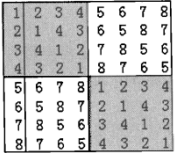
\includegraphics{roundrobin.png}\\
\figcaption{循环赛日程表问题k=3时的解}\label{fig:roundrobin}
\end{center}

\subsubsection{代码}
\begin{Codex}[label=roundrobin_scheduling.c]
#include<stdio.h>
#include<stdlib.h>

#define MAXN 512   /* N=2^k, 0<k9 */
short schedule[MAXN][MAXN];

void dc(const int k) {
    int i, j, t;
    int n, n2; /* 当前的n,即将扩展的n */

    /* k=1,即两个人时,日程表可以直接写出 */
    n=2;
    schedule[0][0]=1; schedule[0][1]=2;
    schedule[1][0]=2; schedule[1][1]=1;

     /* 迭代处理,依次处理2^2....2^k个选手的比赛日程 */
    for(t = 1; t < k; t++, n *= 2) {
        n2 = n * 2;
        //填左下角元素
        for(i = n; i < n2; i++)
            for(j = 0; j < n; j++)
                schedule[i][j] = schedule[i-n][j] + n;

        //将左下角元素抄到右上角
        for(i = 0; i < n; i++)
            for(j = n; j < n2; j++)
                schedule[i][j] = schedule[i+n][j-n];

        //将左上角元素抄到右下角
        for(i = n; i < n2; i++)
            for(j = n;j < n2; j++)
                schedule[i][j] = schedule[i-n][j-n];
    }
}

/* 另一个版本 */
void dc2(const int k) {
    int i, j, r;
    int n;
    const int N = 1 << k;

    /* 第一列是选手的编号 */
    for(i = 0; i < N; i++) schedule[i][0] = i + 1;
    schedule[0][1] = 1;  /* 当 k=0时,只有一个人 */

    for (n = 2; n <= N; n *= 2) {  /* 方块大小, 2, 4, 8 */
        const int half = n / 2;
        for (r = 0; r < N; r += n) { /* 方块所在行 */
            for (i = r; i <= r + half -1; i++) {  /* 左上角小方块的所有行 */
                for (j = 0; j < half; j++) {  /* 左上角小方块的所有行 */
                    /* 右下角 <-- 左上角 */
                    schedule[i + half][j + half] = schedule[i][j];
                    /* 右上角 <-- 左下角 */
                    schedule[i][j + half] = schedule[i + half][j];
                }
            }
        }
    }
}


int main(){
    int k, N;
    int i,j;

    scanf("%d",&k);
    N = 1 << k;

    dc(k);
    // dc2(k);

    // 输出日程表
    for(i = 0; i < N; i++) {
        for(j = 0; j < N; j++) printf("%d ", schedule[i][j]);
        printf("\n");
    }
    return 0;
}
\end{Codex}

\subsubsection{相关的题目}
与本题相同的题目:
\begindot
\item 《算法竞赛入门经典》\footnote{刘汝佳,算法竞赛入门经典,清华大学出版社,2009}第149页8.3.2节
\item 《计算机算法设计与分析(第3版)》\footnote{王晓东, 计算机算法设计与分析(第3版), 电子工业出版社, 2007}第34页2.11节
\item NKOJ 1437 校长杯, \myurl{http://acm.nankai.edu.cn/p1437.html}
\myenddot

与本题相似的题目:
\begindot
\item SPOJ 2826 Round-Robin Scheduling, \myurl{http://www.spoj.com/problems/RRSCHED/}
\item UVa OJ 678 Schedule of Taiwan Baseball League, \myurl{http://t.cn/zHJD9TQ}
\myenddot
